\hfill \newline
\phantom{ } Then we built the summing aplifier circuit according to the figure below. We kept the power supply at $ \mathrm{V_s} = \pm12\si{V} $, and set the function generator to provide ${v_1}(t)=cos(2000\pi t)\si{V}$, ${v_2}(t)={v_3}(t)=0$. All resistors were set to $100\si{k\Omega}$ and the capacitor $C=22\si{pF}$.
\begin{figure}[!htbp]
	\centering 
	\begin{framed}
		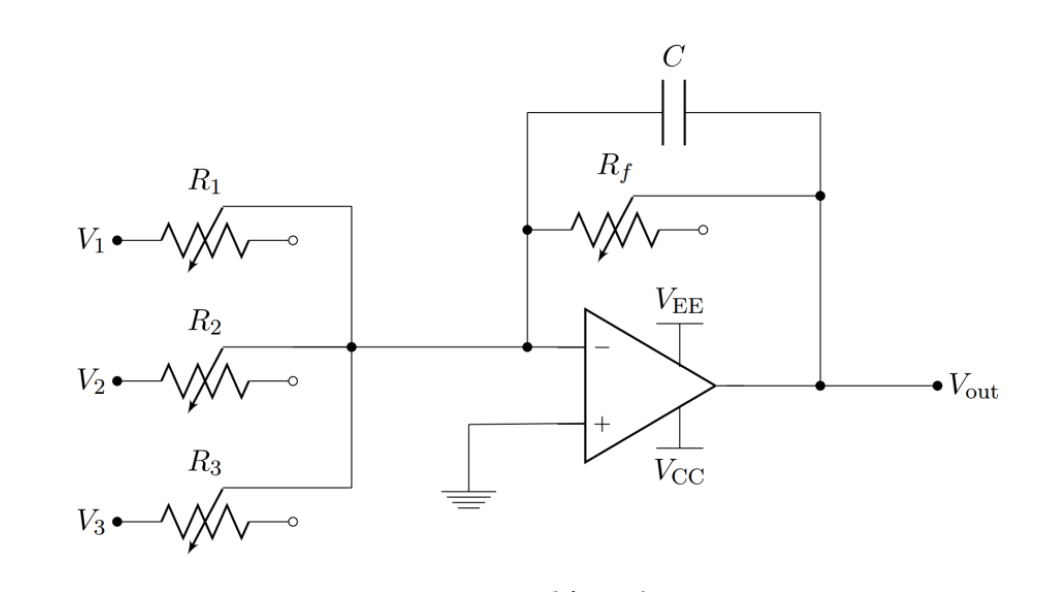
\includegraphics[width=\linewidth]{images/summing_amp.PNG} 
		\caption{Summing amplifier with potentiometers}
		\label{fig:samp} 
	\end{framed}
\end{figure} 

\phantom{ } We swept the frequency of $\mathrm{V_1}$ from 10$\si{\hertz}$ to 1$\si{M\hertz}$, kept the input amplitude same and recorded the amplitude of output signals. The data collected is showed in Table[\ref{tab:caf}], and we got a plotted figure Figure[\ref{fig:afreq}] of the output voltage in terms of frequency.\\

\begin{table}[!htbp]
	\centering
	\caption{Amplitudes under different frequencies}
	\begin{tabular}{lccllcc}
		\toprule
		No&freq($\si{\hertz}$)&Amp($\si{\volt}$)&&No&freq($\si{\hertz}$)  &Amp($\si{\volt}$)\\
		\midrule
		1	&10		&1.94	&&9 &$5*10^3$&2.02\\
		2	&20		&1.94	&&10&$1*10^4$&2\\
		3	&50		&1.94	&&11&$2*10^4$&1.92\\
		4	&100	&1.94	&&12&$5*10^4$&1.55\\
		5	&200	&1.92	&&13&$1*10^5$&1.05\\
		6	&500	&1.96	&&14&$2*10^5$&0.604\\
		7	&1000	&1.96	&&15&$5*10^5$&0.28\\
		8	&2000	&1.98	&&16&$1*10^6$&0.152\\
		\bottomrule
	\end{tabular}
	\label{tab:caf}
\end{table}

\begin{figure}[!htbp]
	\centering 
	\begin{framed}
		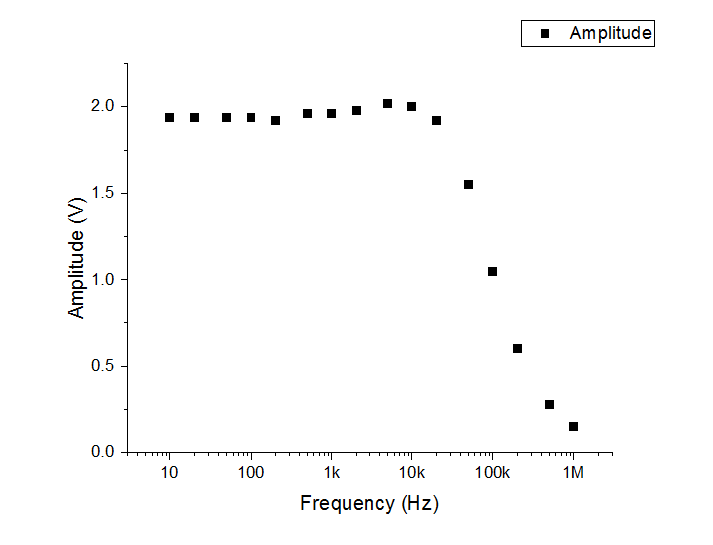
\includegraphics[width=\linewidth]{images/amp_freq.PNG} 
		\caption{Amplitudes under different frequencies}
		\label{fig:afreq} 
	\end{framed}
\end{figure} 

\textbf{Analyze \#4:} \newline
\phantom{ } As we can see, our records are in a similar shape with the theoretical result-relatively flat at high frequency, and starts falling around the frequency of 10$ \si{k\hertz} $. The reason for the three graphs falling in different slope is that the y-axis is in different scales and values.\\
\begin{figure}[!htbp]
	\centering 
	\begin{framed}
		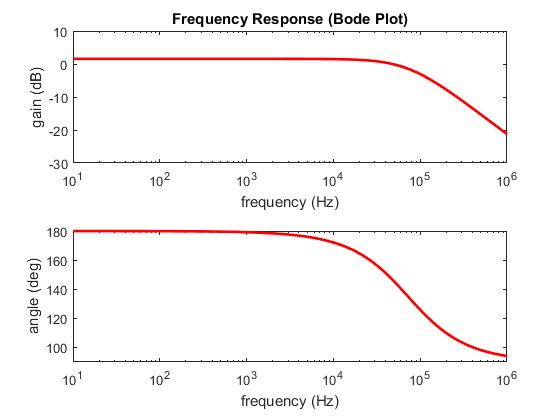
\includegraphics[width=\linewidth]{prelab/images/9_1.PNG} 
		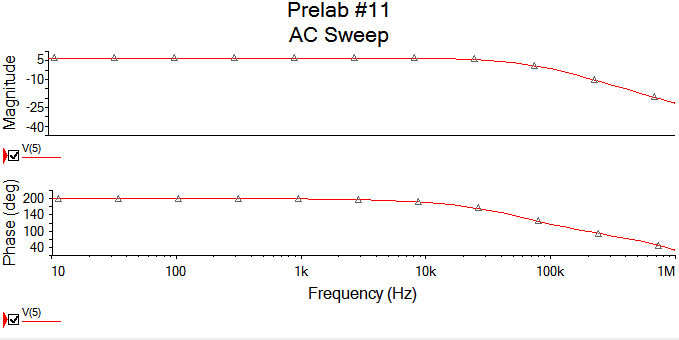
\includegraphics[width=\linewidth]{prelab/images/11_1.PNG}
		\caption{Magnitude and phase of the output signal}
		\label{fig:pre8} 
	\end{framed}
\end{figure} 

\phantom{ } Then we connected a smartphone to the circuit to provide supplemental audio sound as an input signal. The output voltage displayed on the oscilloscope is shown in the figures below.
\begin{figure}[!htbp]
	\centering 
	\begin{framed}
		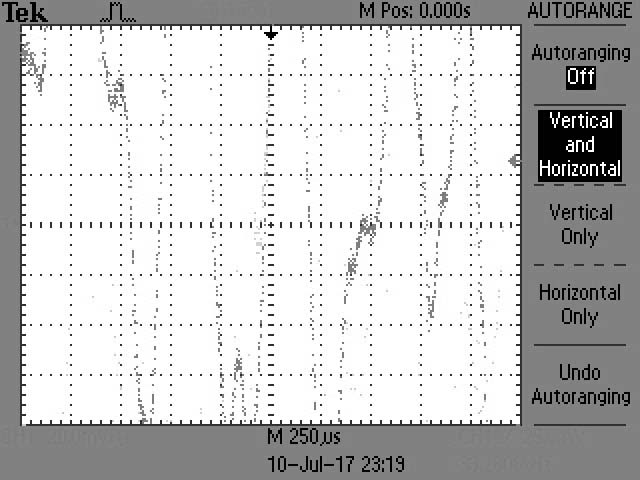
\includegraphics[width=\linewidth]{images/TEK0011.jpg}
		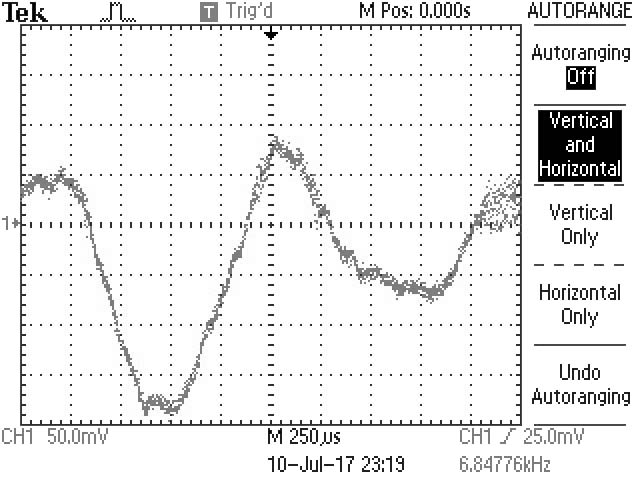
\includegraphics[width=\linewidth]{images/TEK0012.jpg} 
		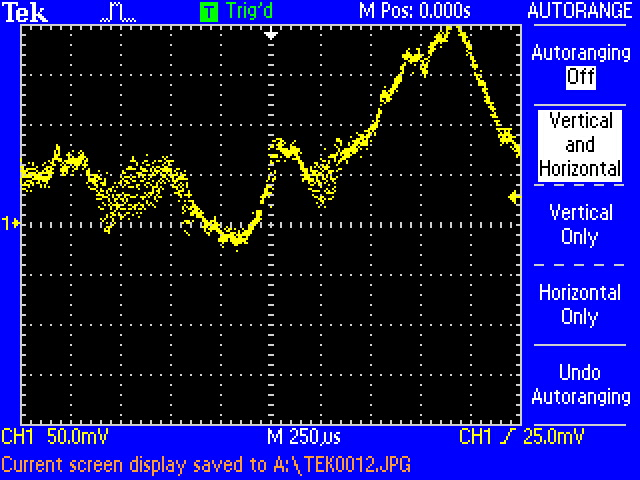
\includegraphics[width=\linewidth]{images/TEK0013.jpg}  
		\caption{The output signals of audio sounds input.}
		\label{fig:pre11} 
	\end{framed}
\end{figure}

\textbf{Analyze \#5:} \newline
\phantom{ } The waveform displayed on the oscilloscope screen was unstable and kept changing, so we provided three screenshots above. Obviously it is not a sine wave, but also not a compelety random signal. Then we used the function generator to provide a 1kHz sine wave, which made a constant sound of a pure tone in the speaker. With a higher frequency the pitch of the sound goes up, and vice versa.

\phantom{ } Next, we used the music in our phones as three input tracks. The output sound was a mix of three music tracks.\\

\textbf{Analyze \#6:} \newline
\phantom{ } When we adjusted the four potentiometers separately, we found that $ \mathrm{R_f} $ controls the whole volume while other three potentiometers controls the volume of each track respectively. The overall volume will decrease when the potentiometer's resistance decreases. Other three potentiometers controls the volume of the sources that they respectively connected to. The volume of the source that goes through one of these three potentiometers will fall when the nearest potentiometer's resistance falls. 